\section{Methods}

\begin{figure*}
\begin{center}
  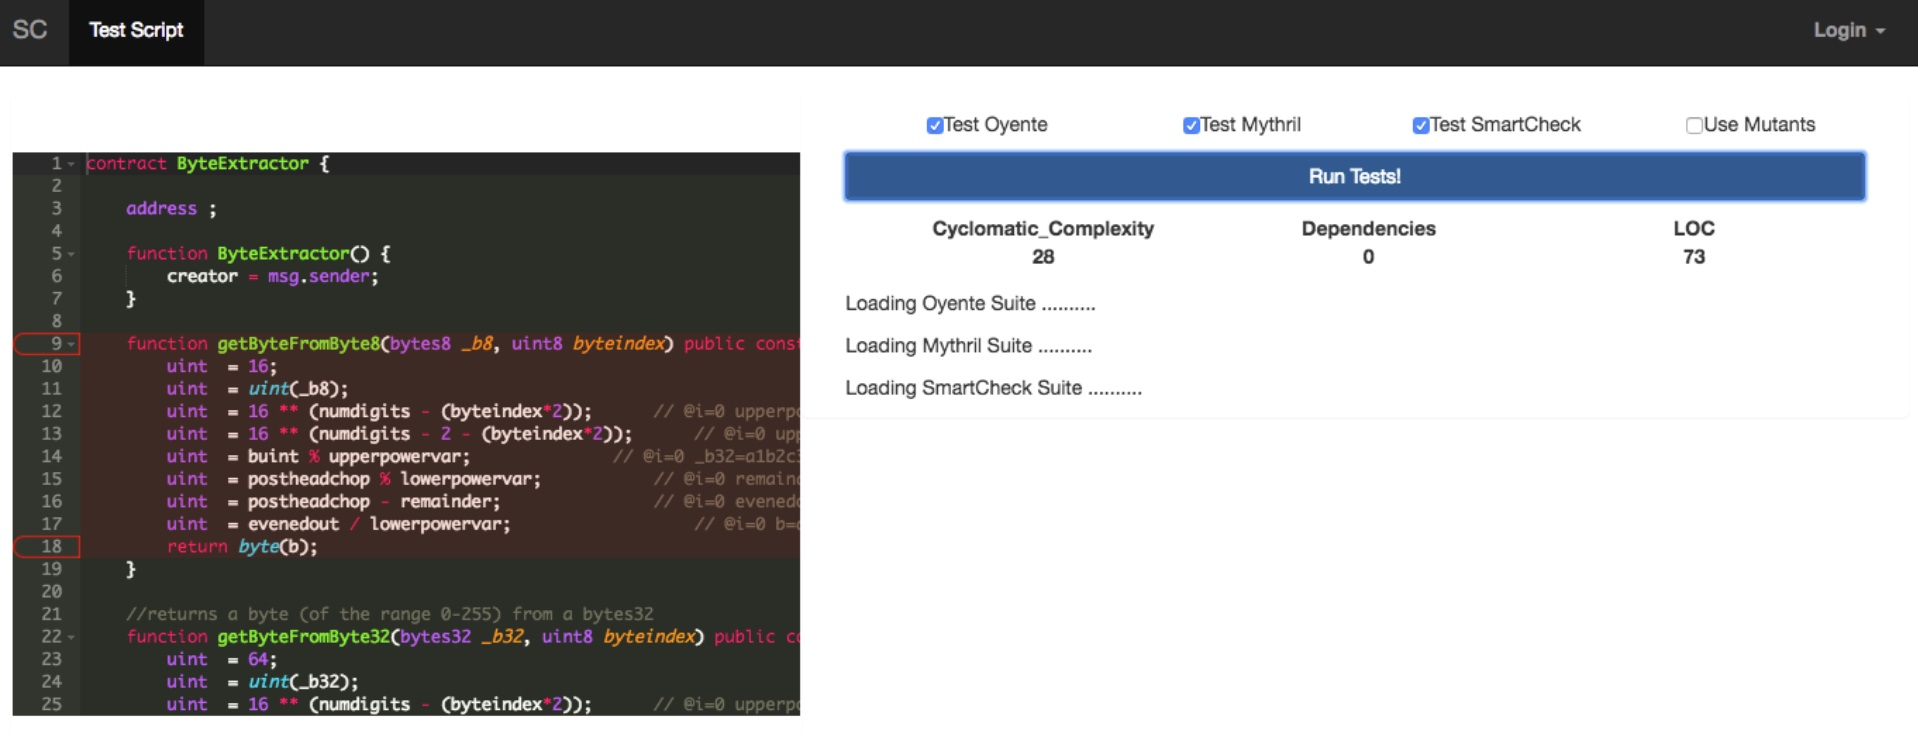
\includegraphics[width=0.9\textwidth]{img/ui1.jpg}
  \label{fig:ui1}
  \caption{The Smarter Smart Contract Testing Tester User Interface}
\end{center}
\end{figure*}

\begin{table}[h!]
%\centering
\begin{tabular}{|cccc|}
\hline
\textbf{Vulnerability}	&\textbf{Oyente}&	\textbf{Mythril} & \textbf{SmartCheck}	\\
\hline
Integer Overflow & yes & yes &  \\
Integer Underflow & yes & yes &  \\
Callstack Depth Attack & yes & yes & \\
Transaction-ordering & yes & yes & yes\\
Re-Entrancy & yes & yes & yes \\
Unprotected Function & & yes & \\
Missing check on return & & yes & \\
Multiple sends & & yes & \\
Complex fallback& & yes & \\
DoS by External Contract & & & yes \\
Gas costly patterns & & & yes \\
Locked Money & & & yes \\
Unchecked external call & & yes & yes \\
Hardcoded address & & & yes \\
Using tx.origin & & yes & yes\\
Costly loop & & & yes \\
Integer division & & & yes \\
Malicious libraries & & & yes \\
Depreciated functions & & yes & \\
\hline
\end{tabular}\\
\label{coverage}
\caption{ Suite coverage of more notable vulnerabilities}
\end{table} 
\subsection{Testing Suites}
\subsection*{Choosing Testing Suites}
While investigating various testing suites, we found that most analysis tools covered similar bugs. As a result, we chose our final testing suites based off of popularity, vulnerability coverage, and ease of use. Out of all analysis tools, Oyente was the most accurate -- it had the lowest false positive/negative rates \cite{ntnutools}. It was also the best for consistency, in that it could analyze source code and bytecode to check for discrepancies. SmartCheck had the widest coverage; its knowledge base is more than double the size of each of the others. Additionally, Oyente, Mythril, and SmartCheck each use a different type of analysis (symbolic, concolic, and static respectively), thus providing a variety of perspectives. Throughout trying other testing suites, many were difficult to set up. They required specific dependencies or operating systems, only worked for certain versions of Solidity, or had an extremely limited feature set. Ultimately, we decided that these three would provide the widest and most accurate coverage for developers using our platform. \\

Furthermore, we found that contracts often violate the same bugs, even if these bugs have induced incredibly expensive errors in the past. As such, these tools' coverages also overlap on the most common bugs. Some examples of these are having integer underflow or overflow, running out of stack frames, re-entrancy, denial of service, being dependent on timestamps or contract execution ordering. Most notably, the re-entrancy attack which was used on the DAO is covered by all three of our testing suites. Other suites we investigated are Manticore, Solgraph, solidity-coverage, Solcheck, Solint, Solium, Solhint, F*, Gasper, and Porosity. Most of these had insignificant coverage or insufficient documentation. A list of our testing suite coverage on the more significant vulnerabilities is in table \ref{coverage} \cite{mythrilvuln, scvuln}. 

\subsubsection{Vulnerability Relevance and Contract Testing}

We chose these bugs because they are well known but still occur in many smart contracts. We checked these vulnerabilities on contracts of all sizes. Some notable contracts are in the repository. The two most well known are Cryptokitties and King of the Ether Throne. Cryptokitties is one of the first blockchain games, where you collect and breed digital cats. Players can breed cats together to create new, unique cats. In December 2017, this game got so popular that it congested the network, causing all time highs in transactions and slow speeds. The most expensive cat bought was 117,712 USD. The Gas limit was even increased in response to Cryptokitties. Next, King of the Ether Throne is a status symbol where you pay a fee to become the king. You must pay more than what the current king previously paid to become the king to knock him off the throne. Yet, there was a vulnerability. By adding a complex fallback that would take a large amount of gas, thus causing the send function to fail, one could claim the throne while not paying the previous king anything. These are both large, well-known contracts, thus giving us a good view into how the tool works with real life contracts.


\subsection*{Oyente}
Oyente works by finding the gap between contract programmers' assumptions about the system and the actual nature of the platform. This gap is the core reason for thousands of bugs on the Ethereum network -- the most popular smart contract platform today. OYENTE uses symbolic execution to analyze Ethereum smart contracts \cite{luu2016making}. \\

As proof of OYENTE's effectiveness, the creators tested 19,366 smart contracts and found that 8,833 contracts have potential bugs. The total value in these contracts was equal to around 30 million USD when they created the tool. Ethereum's value has risen dramatically since. Over the last few years, several vulnerabilities have made headlines worldwide. The most significant of these is TheDAO bug, which had a 60 million loss in USD. If the creators had used OYENTE, they would have caught this bug early on. \\

Some notable bugs Oyente searches for are mishandled exceptions, deliberately hitting the stack limit, timestamp-independent calls, and functions that depend on transaction ordering. The first two are significant because the developer must explicitly implement what happens when a call fails. For instance, in the \texttt{send} function, where people send Ether to someone else, it is fully possible for this function to fail. In response, the developer must revert all that has happened thus far, such as un-withdrawing money from an account. Next, timestamp-independence and transaction ordering are important because miners are allowed to choose what contracts to run. Often times, developers use timestamps as seeds for randomization, but this is easily attacked when miners can determine the seed. This logic applies similarly for transaction ordering. When the result of a contract is dependent on another contract's running before or after it, then miners have influence over the effect of the contract. Thus, the contract is not secure.  \\

Creators of Oyente chose to use symbolic execution, which uses symbols to represent what conditions some combination of variables might satisfy. This was preferable to dynamic testing, which would try much more inputs. This would be even worse than normal in Ethereum, because there could be far more variables on a decentralized network. For instance, in order to check timestamp-ordering independence, the program would have to check every possible variation of race condition caused by multiple programs interacting with each other. \\

More specifically, Oyente has several key components. It simulates the Ethereum Virtual Machine with 4 tools: the CFG Builder, Explorer, CoreAnalysis and Validator. The CFG Builder creates a control flow graph to see which parts of code can jump to others. Some of these edges are generated with symbolic execution, as it may be difficult to determine all the jumps with only static analysis. Next, the Explorer runs through the graph created by the CFG Builder and executes symbolic instructions given a certain state. It runs symbolic instructions for every single state to figure out if branch conditions may be met. At this point, it also adds potential edges to the CFG. After the Explorer runs, we are left with symbolic traces that show what conditions must be satisfied for certain events to occur. To do the actual analysis, we have CoreAnalysis. This runs along the symbolic traces and searches for the various vulnerabilities listed previously. Finally, we have Validator. This looks for false positives. Given the potential execution trees, it checks if the symbolic variables contradict one another. \\

Overall, Oyente is the most accurate tool because of its ability to compare bugs found from comparing source code and from comparing EVM bytecode. 


\subsection*{Mythril}

Another tool similar to Oyente, is Mythril, a security analysis tool specifically for Ethereum smart contracts written in Solidity. It uses concolic execution, or a mix of symbolic and concrete execution, and taint analysis to find which variables take user input (and thus make symbolic), and control flow checking to detect a variety of security vulnerabilities. These vulnerabilities include integer underflow, owner-overwrite-to-Ether-withdrawal, and many others. However, Mythril does not handle any business logic and is therefore not a formal verfication tool. \\

This tool is built on the Ethereum Virtual Machine, or EVM, using the Laser-Ethereum, which is a symbolic interpreter for Ethereum bytecode. The EVM is what allows Mythril to successfully use symbolic execution, as it is much simpler than a desktop or mobile operating system, and thus allows the symbolic execution to reach 100\%  code coverage. With the EVM,  devlopers of Mythril did not have to worry about hard to model features of an Operating System such as filesystems, sockets, or multi-threading. Laser-Ethereum takes in at least one smart contract account as input and returns a set of abstact program states. Each state is made up of the set of values of all the variables in the EVM at a given point in execution. \\

Mythril has many detection modules, including unchecked suicide or ether\_send, unchecked\_retval, external calls to untrusted contracts, integer overflow/underflow, etc. The error of unchecked "suicide" or "self-destruct", which is the act of sending the remaining balance of a contract to a specified user, has been exploited as recently as November 6th, 2017,  on the Parity multisig wallet library contracts, where 280 million dollars worth of Ether was made inaccessable. Mythril has proved to be very effective at detecting this dangerous vulnerability (as well as many other bugs) and will help prevent such attacks in the future by giving developers a chance to test their code for vulnerabilities before deploying their contract.

\subsection*{SmartCheck}
\begin{table*}[ht!]
\centering
\begin{tabular}{|ccp{4.5in}|}
\hline
\textbf{Operation} & \textbf{Mutations} & \textbf{Description} \\
\hline
\texttt{+}  &   \texttt{-}   &   Occurs often when increasing the amount owed, or the amount paid. Can lead to errors associated with loops that end when a balance is paid. \\
\texttt{>}  &   \texttt{<}   &   Can cause limits to be ignored, such as with debate period, leading to errors caused by exceeding maxima.  \\
\texttt{/}  &   \texttt{*}   &   Commonly used during increments of some delta time or delta value measure. Can lead to infinite loops when relying on total value to exceed some measure. \\
\texttt{\&}  &   \texttt{|}   &  Allows checks that require multiple steps to succeed to move forward if only one condition is met. \\
\texttt{==}  &   \texttt{!=}   &   Hard equality checks, such as the 51\% attack check in the example in figure \ref{code:proposal}, will work reverse from intended.\\
\hline
\end{tabular}\\
\label{Mutations}
\caption{ The mutations applied to each script. In this table any instance of the \textbf{Operation} column will be replaced by the \textbf{Mutations} column and vice versa. The descriptions section describes circumstances that would cause more bugs to arise from this mutation. }
\end{table*} 
Finally, the last tool we incorporated was SmartCheck \cite{smartcheck}. This uses static analysis to detect vulnerabilities. SmartCheck detects significantly more vulnerabilities than Oyente and Mythril, likely due to its creators' motivations. Whereas Oyente and Mythril were created as research projects, SmartCheck is a product of SmartDec -- a security company that performs audits contracts for others \cite{smartdec}. \\

When performing an audit, SmartDec asks for relevant solidity files, whitepapers, and anything else the client is willing to provide. It then runs a variety of test suites, including SmartCheck, then manually checks each error or warning to ensure correctness. This allows them as a company to reach a more accurate result than what other tools may do alone, since they can perform custom analysis as well. For instance, in their report for MinerOne, they found that the ICO sale start date specified in the whitepaper differed from what was implemented \cite{minerone}. Furthermore, SmartDec's knowledge base is much larger and updates more quickly because there is a business running behind it. Overall, SmartCheck gives us insight on how professional security analysts investigate contracts. 

\begin{figure}
\begin{center}
  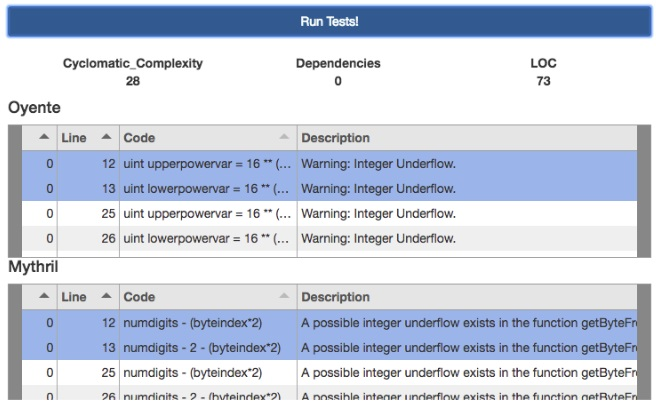
\includegraphics[width=0.5\textwidth]{img/ui2_2.jpg}
  \label{fig:ui2_2}
  \caption{The results of each test suite is highlighted to emphasize tagged code sections.}
\end{center}
\end{figure}

\subsection{User Interface}

To take advantage of the Mythril and Oyente testing suites, we present our user interface that allows running several testing applications and viewing the results interactively in a browser, shown in figure~\ref{fig:ui1}. Users can upload and modify or write a new Solidity Smart Contract in the syntax-highlighted editor, and choose to run Oyente, Mythril, SmartCheck or any combination of the three tools to detect security vulnerabilities in the code. The output is displayed as a verbose list of errors and warnings with exact line numbers identifying the cause of the vulnerability. \\

The application is a web based front-end that can run in any browser, supported by a Python back-end that automatically schedules tasks and prepares environments for each tool individually, reducing the amount of set-up time and knowledge required on behalf of the user to effectively nothing beyond loading a web-page. Additionally, the back-end is able to maintain the environment using docker containers to drastically speed up future runs of the test suites, reducing the overhead time and computational costs of each run after the first from the order of minutes to mere seconds. \\

\begin{figure}
\begin{center}
  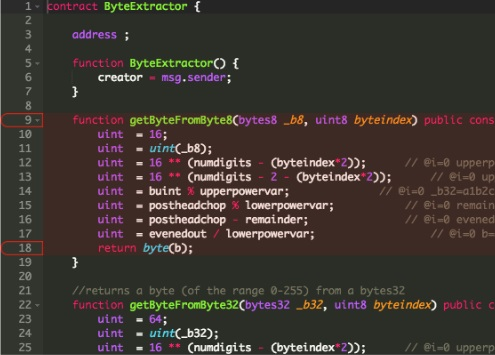
\includegraphics[width=0.5\textwidth]{img/ui2_1.jpg}
  \label{fig:ui2_1}
  \caption{A Smart Contract in the interface can be highlighted with the side-bar, shown here from lines 9 to 18.}
\end{center}
\end{figure}

The interface supports user-defined tagged sections for identifying critical sections of smart contracts. By highlighting, or "tagging," a section of the smart contract, a user can get more specific feedback from the test suites, shown in figure~\ref{fig:ui2_1}. This feature is currently limited to only prioritizing and clarifying information related to the tagged sections of code, shown in figure~\ref{fig:ui2_2}, but in the future could also influence the behavior of tools. For instance, if a tool is timing out while running analysis on the smart contract, we could ensure that it is prioritizing tagged sections and leaving less important sections to be possibly cut short. None of the tools we've tested in this work, however, face the issue of timing out while analyzing reasonable length smart contracts, so this feature would not be useful with the current implementation. \\

Portability and accessibility are achieved through Docker containers that are managed by the API. Each container has the necessary environment and dependencies, automatically fetching them from a trusted repository, so that even running locally, the tool requires minimal set-up. While it can be run locally, the application as a whole is intended to be used entirely web-based, uploading the Smart Contract to a remote server for testing and returning the results within a browser window. \\

Our solution covers several use cases, primarily those of the Smart Contract writer, the second party to a contract, as well as reviewers of the implemented test-suites. The Smart Contract writer is able to interactively view vulnerabilities in her code and quickly make iterative changes with the built-in and fully syntax-aware code editor window. The second party, assumed to be ignorant of the finer points of Smart Contracts, including how to write them, is able to verify security and integrity without having to learn from scratch how to run any of these complicated test suites on his own. Finally, a reviewer can take contracts with known or unknown flaws and compare the outputs of multiple tools to test which produces the best or most accurate output. \\

This user interface is designed and used not only for our study to measure the ability of Oyente, Mythril and SmartCheck to detect security flaws, but also for the public to use to have easily accessible testing capabilities for any Smart Contract written in Solidity. With this tool, testing a Solidity Smart Contract is easy and straightforward, since the entire process from fetching dependencies all the way to destroying the containers on completion is managed totally automatically. This end-to-end approach is intended to make it possible for a lay-person to engage in a Smart Contract knowing that it has been tested by the best open-source tools available, while still providing the important technical information that the contract writer needs to create a sound and error-free contract. \\

     
\begin{table*}[h!]
\centering
\begin{tabular}{|ccccccc|}
\hline
 & & \textbf{Cyclomatic Complexity}	&\textbf{Dependencies}&	LOC	&	\textbf{\# Errors} &	\textbf{\# Issues} \\

\hline
SmartCheck & Original  & 16.07 & 0.302 & 81.613   & 4.316 & \\
        & Mutated  & 44.249 & 0.444 & 81.613   & 5.348 & \\
 Oyente & Original   & 16.07 & 0.302 & 81.613  & 2.442 & 10.535\\
        & Mutated  & 44.249 & 0.444 & 81.613 &  5.026 & 0.9\\
Mythril & Original  & 16.07 & 0.302 & 81.613 &   0.977 & 5.767\\
        & Mutated  & 44.249 & 0.444 & 81.613 &   1.077 & 3.209\\
\hline
\end{tabular}\\
\label{tbl:Statistics}
\caption{ The statistical analysis of the different test suits for both the original and mutated scripts. This shows that SmartCheck detects the most bugs, followed by Oyente, and then Mythril. Moreover, this is much more pronounced with the mutated scripts. Note, SmartCheck did not provide meaningful warnings and thus has no associated Issues column.}
\end{table*} 

\subsection{Analysis Techniques}
\subsection*{Mutation Studies}
\begin{figure}[h!]
\lstinputlisting[language=C]{code/proposal.txt} 
\label{code:proposal}
\caption{Example script from the DAO smart contract codebase.}
\end{figure}
To expand upon the testing suites, we added mutations to the Solidity scripts to compare which suites would recognize that these perturbations. To create these mutations we replaced standard operations with contrary logic while avoiding syntactical errors. With these changes, we ran the testing suites again on the altered scripts. \\

The mutations were applied as a search and replace of a single operation per test. Thus, a file containing 10 unique operations would produce 10 mutated files each with a single operation mutated. For the mutations, we chose operations that would reverse the logic of the of the given statement. For example, consider the block of code from the DAO smart contract in Figure \ref{code:proposal}. \\

In this example, there is a list of checks that are made prior to scheduling a contract between a \texttt{sender} and \texttt{recipient}. Specifically, the receiving party is first checked against a list of allowed recipients, the debating period, or time frame to cancel the contract, is confirmed to be in a predefined range, that enough money has been deposited to cover this transaction, and importantly a check against a 51\% attack, where a majority owner of the block chain can cheat the system, is protected against. A valid testing suite should recognize the insecurities presented if any one of this statements is not checked. Thus our mutations primarily change the logic in checks like the one above. A simple way to guarantee this is by reversing the logic on each operation. For example the check against a 51\% attack relies on a equality constraint, thus if this changed to an inequality we can guarantee that check will fail. A complete list of the mutations made on each Solidity script is  given in table \ref{Mutations}. \\
     
\subsection*{Static Analysis}

In addition to Mutation studies, we also performed static analysis on the solidity scripts to provide metrics to help explain why one suite performed better than another. These metrics include measuring the number of lines, complexity, and dependencies in a block of code. These metrics were chosen following the results of Kochnar et al.'s code coverage study \cite{kochhar2017code}. \\

The statistical measures used to analysis the solidity script were Lines of Code (LOC), Cyclomatic Complexity, and the number of Dependencies. Lines of Code was directly computed from each script after removing whitespace and comments. One limitation of this measure, is that it does not account for varying coding styles, such as placing brackets in line with function signatures, but overall this provided a good metric for length of a script. Cyclomatic Complexity measure the dependence between certain paths within a block of code. This metric increases by one at each point where a new branch will need to be tested; such as an if statement or logical decision \cite{mccabe1976complexity}. Dependencies measures the number of imports into a script, causing this file to require correct execution of the dependent file. For example a DAO solidity package consists of many separate scripts that each import a base DAO class. Thus each of these would have a dependency of at least 1. With these measures, we were able to balance the testing suite results with concrete information that can easily be pulled from a script; allowing for breadth in our study. \\


